\subsection{Vorbereitung der Daten und deskriptive Analysen}
Die erhobenen Daten wurden mittels SPSS Version 25 für Mac OS X aufbereitet. Die Stichprobendaten wurden direkt aus der Enterprise Feedback Suite \cite{Questback2018} mittels Datenexport für SPSS exportiert. Allfällige Fehlerquellen wurden bei der Datenbereinigung korrigiert. Dies wurde durch die Umfragesoftware erleichtert, indem nur abgeschlossene Datensätze exportiert wurden und eine erste Werteprüfung bereits bei der Eingabe erfolgte (z.B.: es wurden nur Zahlen bei der Eingabe des Jahrgangs zugelassen). Fehlende Werte wurden bereits von der Umfragesoftware gesetzt und konnten innerhalb von SPSS mit einem Wertelabel versehen werden. Für die Berechnung der Mediennutzung, der Bindung, des Stressniveaus und des subjektiven Wohlbefindens wurden zusätzliche Variablen in SPSS erstellt und anhand der generierten Daten berechnet (für die Formel der Berechnung siehe Sektion \textit{\nameref{sec:Design}}).

\subsubsection{Medien und Mediennutzung}
Im Rahmen der Umfrage wurde die Mediennutzung während der Betreuung der Kinder erhoben. Dabei wurde zwischen \textit{privat genutzt}, \textit{geschäftlich genutzt}, \textit{privat \& geschäftlich genutzt} und \textit{nicht genutzt} unterschieden. In Folge der Übersichtlichkeit wurde in \textit{Abbildung \ref{fig:Mediennutzung}} die Ausprägung auf \textit{genutzt} und \textit{nicht genutzt} zusammengefasst, wobei die geschäftliche und die private Nutzung zusammengefasst wurde (für eine detaillierte Darstellung siehe Anhang \ref{app:Mediennutzung}, \textit{Abbildung \ref{fig:AppMediennutzung}}).

97.2\% der Befragten gaben an, das Smartphone während der Betreuung zu benutzen, wobei dies zu 72\% privat, 1.4\% geschäftlich und zu 23.9\% privat \& geschäftlich erfolgte. 2.8\% benutzte das Smartphone während der Betreuung nicht. 31.7\% gaben an, den Fernseher privat zu nutzen und 68.3\% gaben an, den Fernseher nicht zu nutzen. Den Computer (Laptop- oder Desktopcomputer) nutzten 42.4\%, unterteilt in 17.4\% privat, 6.4\% geschäftlich und 18.3\% privat \& geschäftlich. 57.8\% nutzte keinen Computer während der Betreuung. Das Tablet nutzten 19.7\% während der Betreuung (17\% privat, 0\% geschäftlich und 2.8\% privat \& geschäftlich). 80.3\% nutzten das Tablet nicht. Den Radio (Stereoanlage, CD Player) nutzten 62.8\% hautpsächlich privat (57.3\% privat, 1.4\% geschäftlich, 4.1\% privat \& geschäftlich). 37.2\% nutzte den Radio nicht. Printmedien (Buch, Zeitung, Heft, Comic) wurden von 68.8\% genutzt (58.7\% privat, 1.8\% geschäftlich und 8.3\% privat \& geschäftlich) und von 31.2\% nicht genutzt. Foto- oder Videokamera nutzten 55\%, wobei der Hauptanteil von 51.8\% im privaten Rahmen stattfand (0\% geschäftlich und 3.2\% privat \& geschäftlich). Die Spielkonsole wurde von 4.1\% privat genutzt, gegenüber 95.9\%, die sie nicht benutzte. Der MP3 Player wurde von 8.3\% genutzt, unterteilt in 7.3\% private, 0\% geschäftliche und 0.9\% private \& geschäftliche Nutzung. 91.7\% nutzte den MP3 Player nicht während der Betreuung.

% Figure
\begin{figure}[t]
\caption{Medien \& Mediennutzung}\label{fig:Mediennutzung}
\centering
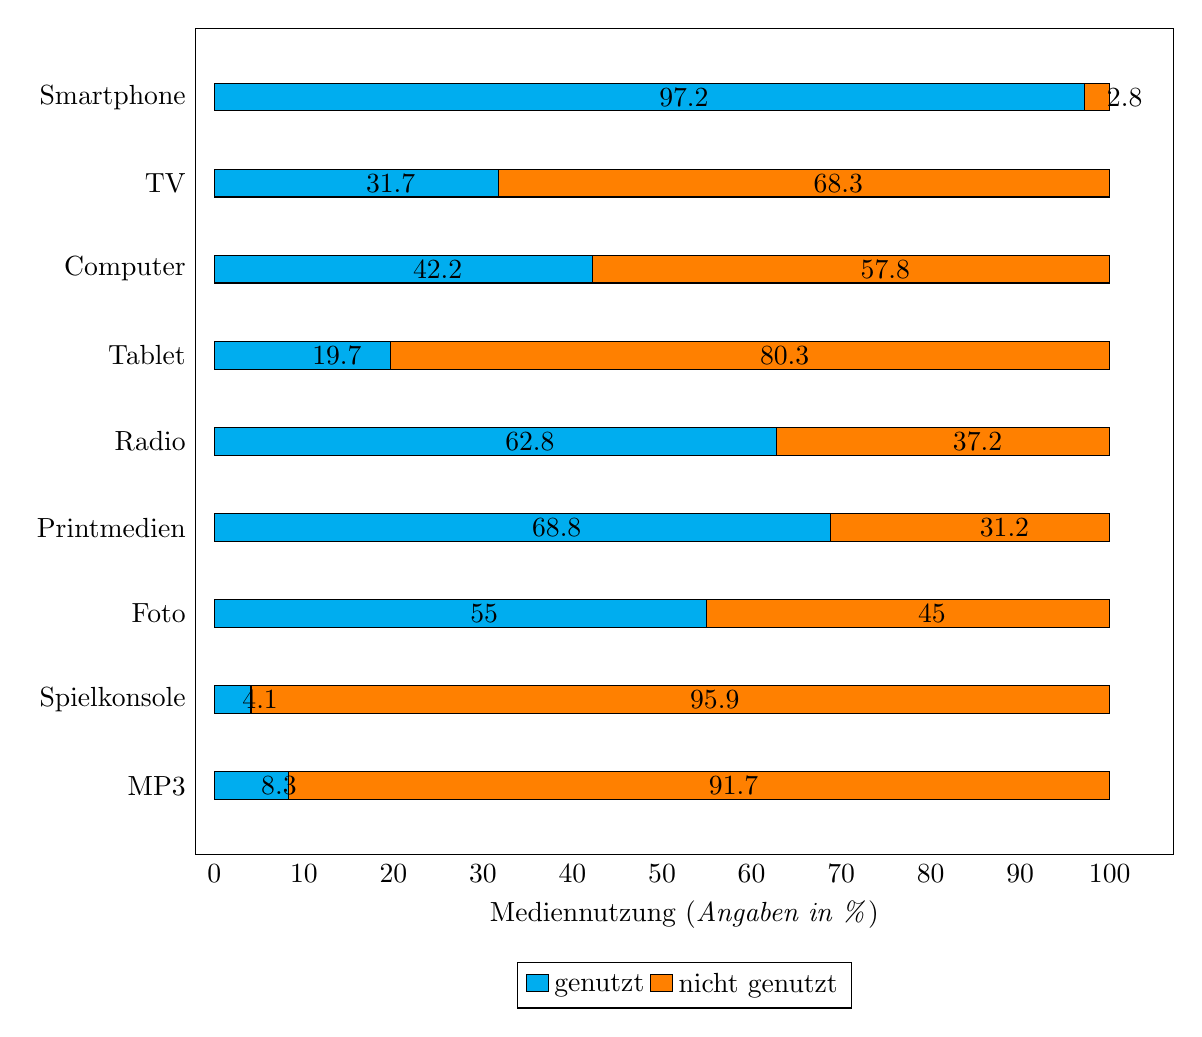
\begin{tikzpicture}[scale=1, auto,swap]
  \begin{axis}[
    xbar stacked,
    %y axis line style = { opacity = 0 },
    %axis x line       = none,
    tickwidth         = 0pt,
    xmin              = 0,
    xmax              = 105,
    enlarge y limits  = 0.1,
    enlarge x limits  = 0.02,
    %/legend pos=south east,
    legend style={at={(0.5,-0.13)}, anchor = north},
    legend columns     = -1,
    %reverse legend,
    ytick             = data,
    xlabel            = {Mediennutzung (\textit{Angaben in \%})},
    %height            = 20cm,
    width             = 14cm,
    symbolic y coords = {MP3, Spielkonsole, Foto, Printmedien, Radio, Tablet, Computer, TV, Smartphone},
    nodes near coords,
    nodes near coords align={horizontal},
  ]
  %benutzt
  \addplot[draw=black,fill=cyan] coordinates { (97.2,Smartphone)(31.7,TV)(42.2,Computer)(19.7,Tablet)(62.8,Radio)(68.8,Printmedien)(55,Foto)(4.1,Spielkonsole)(8.3,MP3)};
  \addlegendentry{genutzt~}
  %nicht genutzt
  \addplot[draw=black,fill=orange] coordinates { (2.8,Smartphone)(68.3,TV)(57.8,Computer)(80.3,Tablet)(37.2,Radio)(31.2,Printmedien)(45,Foto)(95.9,Spielkonsole)(91.7,MP3)};
  \addlegendentry{nicht genutzt}
  
  \end{axis}
\end{tikzpicture}
\end{figure}

Weiter wurde die Medientätigkeit in Minuten anhand der letzten Betreuung des Kindes erfasst (siehe \textit{Tabelle \ref{table:Medientätigkeit}}). Dabei wurde unterschieden, ob das Kind wach war $MSN_{Wach}$ oder geschlafen hat $MSN_{Schlafend}$. Alle Medientätigkeiten summiert ergab den Mittelwert der Nutzung. Dieser belief sich währendem das Kind wach war auf $M$=93.1 Minuten ($SD$=103.6, $Min$=0, $Max$=613) und $M$=108.6 Minuten, währendem das Kind geschlafen hat ($SD$=105.3, $Min$=0, $Max$=495). Total waren die Teilnehmer im Schnitt $M$=202.1 Minuten mit Medien beschäftigt, währendem sie ihr Kind betreuten ($SD$=174.9, $Min$=3, $Max$=840).

%Table
\begin{table}[b]
\begin{tabular}{m{8em} m{4em}  m{4em}  m{5em} m{4em}} 
  \hline
  & $M$ & $SD$ & Min - Max & Schiefe\\
  \hline
  $MNS_{Wach}$* & 93.08 & 103.61 & 0 - 613 & 2.26\\
  $MNS_{Schlafend}$** & 108.63 & 105.32 & 0 - 495 & 1.56\\
  $MNS_{Total}$*** & 202.10 & 174.86 & 3 - 840 & 1.44 \\
  \hline
  \multicolumn{5}{l}{\textit{Anmerkung. *$N$=208, **$N$=205, ***$N$=204, Angaben in Minuten.}}\\
  &&&&\\
\end{tabular}
\caption{Medientätigkeit während der Betreuung}
\label{table:Medientätigkeit}
\end{table}

Auf die einzelnen Medien verteilt bedeutet, dass die Probanden im Schnitt $M_{w}$=5.2 Minuten telefonierten, während dem das Kind wach war und $M_{s}$=7.2 Minuten, währendem das Kind geschlafen hat (siehe dazu \textit{Abbildung \ref{fig:Medientätigkeit}}). Im Schnitt haben die Teilnehmer $M_{w}$=10 Minuten mit Textnachrichten verbracht (lesen und schreiben) währendem das Kind war wach und $M_{s}$=13.8 Minuten währendem das Kind geschlafen hat. Für das bearbeiten und Lesen von Emails setzten die Teilnehmer $M_{w}$=1.7 Minuten (Kind war wach) und $M_{s}$=7 Minuten ein (Kind hat geschlafen). Beim Lesen und Anschauen von Printemedien ((Bilder-)Bücher, Magazinen, Zeitungen, Comics, etc.) setzten die Eltern $M_{w}$=5.3 und $M_{s}$=12.5 Minuten ein. Im Internet verbrachten sie $M_{w}$=5.9 und $M_{s}$=19.7 Minuten mit Surfen und Informationen suchen. Musik hörten die Eltern während der Betreuung $M_{w}$=18.6 und $M_{s}$=8.3 Minuten. Sie schauten im Schnitt $M_{w}$=5.4 und $M_{s}$=25.1 Minuten Fernseher oder Videos (TV-Sender, Netflix, DVD, etc.). Der Radio lief während $M_{w}$=34.3 und $M_{s}$=12.9 Minuten. Fotos oder Videos wurden während $M_{w}$=5.1 und $M_{s}$=0.9 Minuten gemacht. Video-Games (Smartphone, Computer, Konsole, etc.) wurden während $M_{w}$=.2 und $M_{s}$=1.5 Minuten gespielt. Hörspiele und Hörbücher wurden während $M_{w}$=1.5 und $M_{s}$=2.1 Minuten gehört. Die komplette Auflistung der Mittelwerte (wach \& schlafend), inklusive Angabe des  Mittelwerts ist in \textit{Tabelle \ref{fig:AppMedientätigkeit}} im Anhang \ref{app:Medientätigkeit} zu finden.

\begin{figure}%[htp]
\caption{Mittelwerte der Medientätigkeiten während der Betreuung}\label{fig:Medientätigkeit}
%\centering
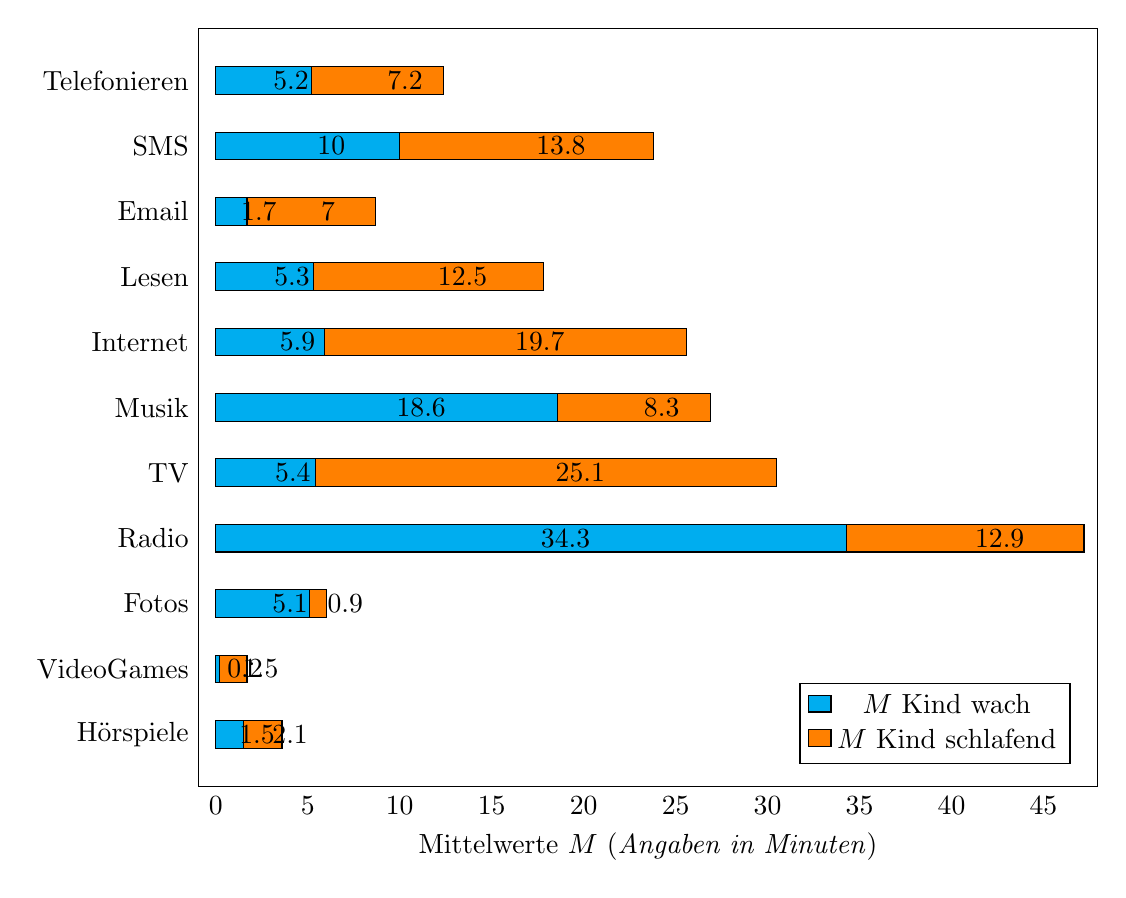
\begin{tikzpicture}[scale=1]
  \begin{axis}[
    xbar stacked,
    %y axis line style = { opacity = 0 },
    %axis x line       = none,
    tickwidth         = 0pt,
    xmin              = 0,
    xmax              = 47,
    enlarge y limits  = 0.08,
    enlarge x limits  = 0.02,
    legend pos=south east,
    ytick             = data,
    xlabel            = {Mittelwerte $M$ (\textit{Angaben in Minuten})},
    %height            = 20cm,
    width             = 13cm,
    symbolic y coords = {Hörspiele, VideoGames, Fotos, Radio, TV, Musik, Internet, Lesen, Email, SMS, Telefonieren},
    nodes near coords,
    nodes near coords align={horizontal},
  ]
  %wach
  \addplot[draw=black,fill=cyan] coordinates { (5.2,Telefonieren)(10,SMS)(1.7,Email)(5.3,Lesen)(5.9,Internet)(18.6,Musik)(5.4,TV)(34.3,Radio)(5.1,Fotos)(.2,VideoGames)(1.5,Hörspiele)};
  
  %schlafend
  \addplot[draw=black,fill=orange] coordinates { (7.2,Telefonieren)(13.8,SMS)(7,Email)(12.5,Lesen)(19.7,Internet)(8.3,Musik)(25.1,TV)(12.9,Radio)(0.9,Fotos)(1.5,VideoGames)(2.1,Hörspiele)};
  
  \legend{\text{$M$ Kind wach}, \text{$M$ Kind schlafend}}
  \end{axis}
\end{tikzpicture}
\end{figure}

Neben der Mediennutzung und der Medientätigkeit wurde die Anzahl Geräte im Haushalt erfragt (detaillierte Auflistung siehe \textit{Tabelle \ref{fig:AppGeräteHaushalt}} im Anhang \ref{app:Mediengeräte}). Dabei gaben 83.9\% der Teilnehmer an, 2 Smartphones im Haushalt zu besitzen. 70.2\% gaben an, ein TV-Gerät zu besitzen. 45\% der Befragten besitzen 2 Computer (Desktop oder Laptop), 45.9\% ein Tablet und 48.2\% einen Radio (Stereoanlage, CD-Player) im Haushalt. 51.4\% gaben an, keine Tageszeitung oder ein Magazins abboniert zu haben. 45.9\% gaben an, einen Fotoapparat oder Videokamera zu besitzen. 61\% besitzen keine Spielekonsole und 67\% keinen MP3 Player.

Zudem wurden die Medien erhoben, auf welche die Eltern während der Betreuung am wenigsten verzichten konnten (siehe \textit{Tabelle \ref{fig:AppMedienverzicht}} im Anhang \ref{app:Medienverzicht}). 85.3\% gaben an, nicht auf das Smartphone verzichten zu können, gefolgt vom Radio (Stereonalage, CD-Player) von 33.9\% und 25.2\% Foto- und Videokamera. Weiter gaben die Teilnehmer an, dass 11.9\% von ihnen nicht auf den Fernseher, 9.6\% nicht auf das Abo einer Tageszeitung oder Zeitschrift, 8.3\% nicht auf den Computer (Laptop oder Desktop), 2.8\% nicht auf den MP3-Player, 2.3\% nicht auf das Tablet und .9\% nicht auf die Spielkonsole verzichten können.

\subsubsection{Bindung anhand AAS}
Die Skalenauswertung des Adult Attachment Scale (\acrshort{aas}) lieferte folgende Werte (siehe \textit{Tabelle \ref{table:AASDeskriptivTrans}}). Dabei wurden die transformierten Skalen mit einem Wertebereich von 0 bis 100 verwendet (siehe dazu die Formel \ref{eq:AASIndexTrans} in Kapitel \nameref{sec:AAS}). Der Mittelwert $M$ der Skala $AAS_{\textnormal{Nähe}}$ beträgt 78.46 ($SD$=15.98). Der Mittelwert $M$ der Skala $AAS_{Vertrauen}$ beträgt 80.18 ($SD$=16.98) und der Mittelwert  $M$ der Skala $AAS_{Angst}$ beträgt 20.28 ($SD$=17.43). Die entsprechenden Werte der original Skalen sind in \textit{Tabelle \ref{table:AppAASDeskriptiv}} in Anhang \ref{app:TablesAas} zu finden.

%Table
\begin{table}%[ht]
\begin{tabular}{m{7em} m{3em}  m{3em}  m{5em} m{3em}} 
  \hline
  & $M$ & $SD$ & Min - Max & Schiefe\\
  \hline
  $AAS_{\textit{\textnormal{NäheTrans}}}$ & 78.46 & 15.98 & 25 - 100 & -.59\\
  $AAS_{VertrauenTrans}$ & 80.18 & 16.98 & 16.67 - 100 & -1.17\\
  $AAS_{AngstTrans}$ & 20.28 & 17.43 & -5 - 75 & .91 \\
  \hline
  \multicolumn{5}{l}{\textit{Anmerkung. $N$=217, Wertebereich Skala 0 bis 100.}}\\
  &&&&\\
\end{tabular}
\caption{Transformierte Skalenwerte der Adult Attachment Scale - AAS}
\label{table:AASDeskriptivTrans}
\end{table}

Für die Beantwortung der Fragestellung wurde anhand der Skalen eine Aufteilung der Stichprobe in sicher und unsicher gebundene Personen vorgenommen. Wie bereits in Kapitel \titleref{sec:AAS} beschrieben, kann eine Aufteilung in das Cluster \enquote{sicher} vorgenommen werden \cite{Schuetzmann2004}. Gemäss dieser Aufteilung lassen sich 69.7\% ($N$=144) der Probanden in sicher und 30.3\% ($N$=60) in unsicher gebundene Personen zuordnen. 

\subsubsection{Stress anhand PSQ}
Die Skalenauswertung des Perceived Stress Questionnaire (\acrshort{psq}) liefert folgende Werte (siehe \textit{Tabelle \ref{table:PSQDeskriptiv}}). Der Mittelwert $M$ der Skala $PSQ_{Sorgen}$ beträgt 24.28 ($SD$=17.69). Der Mittelwert $M$ der Skala $PSQ_{Anspannung}$ beträgt 42.14 ($SD$=21.96). Der Mittelwert $M$ der Skala $PSQ_{Freude}$ beträgt 65.26 ($SD$=19.08). Der Mittelwert $M$ der Skala $PSQ_{Anforderung}$ beträgt 46.97 ($SD$=19.54) und der Gesamtmittelwert $M$ der Skala $PSQ_{Gesamtscore}$ beträgt 37.03 ($SD$=17.11).

%Table
\begin{table}[ht]
\begin{tabular}{m{6em} m{3em}  m{3em}  m{5em} m{3em}} 
  \hline
  & $M$ & $SD$ & Min - Max & Schiefe\\
  \hline
  $PSQ_{Sorgen}$ & 24.28 & 17.69 & 0 - 86.67 & .84 \\
  $PSQ_{Anspannung}$ & 42.14 & 21.96 & 0 - 100 & .26\\
  $PSQ_{Freude}$ & 65.26 & 19.08 & 6.67 - 100 & -.14\\
  $PSQ_{Anforderung}$ & 46.97 & 19.54 & 0 - 100 & .37 \\
  $PSQ_{Gesamtscore}$ & 37.03 & 17.11 & 3.33 - 91.67 & .42\\
  \hline
  \multicolumn{5}{l}{\textit{Anmerkung.} $N$=218, Skala Wertebereich 0 bis 100}\\
  &&&&\\
\end{tabular}
\caption{Skalenwerte des Perceived Stress Questionnaire - PSQ}
\label{table:PSQDeskriptiv}
\end{table}


\subsubsection{Wohlbefinden anhand SHS}
Der Indexwert der Subjective Happiness Scale (\acrshort{shs}) $SHS~I$ beläuft sich in dieser Stichprobe auf $M$ 5.53 ($SD$=1.01) (siehe \textit{Tabelle \ref{table:SHSDeskriptiv}}).

%Table
\begin{table}[ht]
\begin{tabular}{m{6em} m{3em}  m{3em}  m{5em} m{3em}} 
  \hline
  & $M$ & $SD$ & Min - Max & Schiefe\\
  \hline
  $SHS~I$ & 5.53 & 1.01 & 2.25 - 7.0 & -.77 \\
  \hline
  \multicolumn{5}{l}{\textit{Anmerkung.} $N$=218, Skala Wertebereich 1 bis 7}\\
  &&&&\\
\end{tabular}
\caption{Skalenwerte des Subjective Happiness Scale - SHS}
\label{table:SHSDeskriptiv}
\end{table}

% ---------------------------------------
\subsection{Hypothesentest} \label{sec:Hypothesentest}
In diesem Kapitel werden die Hypothesen eins bis vier der Reihe nach überprüft. Die für die Prüfung der Voraussetzung der einzelnen Berechnungsvarianten notwendigen Grafiken (z.B. Histogramme und Q-Q-Plots) wurden aus Platzgründen in den Anhang verschoben (siehe Anhang \ref{app:Hypothesentest_1}).

\subsubsection{Hypothesentest 1}\label{sec:Hypothesentest1}
Für die Überprüfung der Hypothese 1 wurde eine einfaktoriellen Varianzanalyse berechnet, um zu untersuchen, ob es einen Unterschied in der Mediennutzung abhängig zur Bindung gab. Die Bindung wurde in zwei Gruppen unterteilt: Gruppe sicher Gebundene ($N$=144, $M$=199.09, $SD$=179.017) und unsicher Gebundene ($N$=60, $M$=209.316, $SD$=165.701). Die Prüfung auf Normalveteilung mittels Shapiro-Wilks-Test \cite{Shapiro1965} viel signifikant aus (Shapiro-Wilks-Test $p_{sicher}$ = .000, $p_{unsicher}$ = .000 bei $\alpha$ = .05). Der Sichtvergleich mittels Histogramm und Q-Q-Plots zeigten ein ähnliches Bild (siehe Anhang \ref{app:Hypothesentest_1}). Somit kann von einer Abweichung von der Normalverteilung ausgegangen werden \cite{Hemmerich2018} und eine Voraussetzung der einfaktoriellen Varianzanalyse ist verletzt. Gemäss \citeA{UniversitatZurich2018} sind Verletzungen ab einer Gruppe von 25 Probanden in der Regel unproblematisch. Da sich die Gruppe sichererer Probanden aus $N$=144 und die Gruppe unsicher Probanden aus $N$=60 zusammensetzten, wurde die Berechnung weiter geführt.

Gemäss Boxplot wurden zudem Ausreisser im Datensatz festgestellt (siehe Anhang \ref{app:Hypothesentest_1}). Für die Gruppe unsicher Gebundenen kann ein Fall mit der Id 38 identifiziert werden, der 1.5 Standardabweichungen vom Mittelwert entfernt ist. Bei der Gruppe sicher Gebunden waren es sieben Fälle (12, 30, 39, 48, 115, 165, 205). Die Varianzanalyse ist gegenüber Ausreissern nur bedingt robust \cite{Hemmerich2018}. Das es sich in diesem Fall um leichte Ausreisser handelte, wurden sie im Datensatz belassen und die Berechnung mit ihnen weitergeführt.  

Die Überprüfung der Varianzhomogenität erfolgte mit dem Levene-Test, gemäß dem wir eine Gleichheit der Varianzen annehmen können (Levene-Test; $p$ = .683). 

Der Hypothesentest für Hypothese 1 mittels ANOVA liefert ein nicht-signifikantes Ergebnis. Die Bindung von sicher und unsicher gab keinen statistisch signifikanten Unterschied auf die gesamte Mediennutzung der Stichprobe ($F$(1,202) = .144, $p$=.704, partielles $\eta^2$=.001, $n$=204). Basierend auf diesen Ergebnissen muss die Nullhypothese $H1_{0}$ angenommen werden. 

\subsubsection{Hypothesentest 2}
Für die Überprüfung der Hypothese 2 wurde eine einfache lineare Regression durchgeführt, um zu untersuchen, inwiefern sich die Mediennutzung (Kriterium) durch den Prädiktor Stress vorhersagen lässt.

Für die Prüfung der linearen Beziehung zwischen der abhängigen und der unabhängigen Variable wurde ein Streudiagramm erstellt (siehe \textit{Abbildung \nameref{fig:AppStreudiagrammMedienPsq}} in Anhang \ref{app:Hypothesentest_1}). Darin ist praktisch keine Beziehung zwischen den Variablen zu erkennen.

Der Hypothesentest für die Hypothese 2 mittels einfacher linearer Regression liefert ein nicht signifikantes Ergebnis. Das Stressempfinden der Eltern geht somit nicht mit einer höheren Mediennutzung einher (F(1,202) = .389, $p$=.533). Die Nullhypothese $H2_{0}$ muss angenommen werden.

\subsubsection{Hypothesentest 3}
Für die Überprüfung der Hypothese 2 wurde eine einfache lineare Regression durchgeführt, um zu untersuchen, inwiefern sich das subjektive Wohlbefinden (Kriterium) durch den Prädiktor Mediennutzung vorhersagen lässt.

Der Hypothesentest für die Hypothese 3 mittels einfacher linearer Regression liefert ein nicht signifikantes Ergebnis. Es gibt keinen statistischen Zusammenhang zwischen dem Stressempfinden und dem subjektiven Wohlbefinden der Stichprobe (F(1,202) = 1.837, $p$=.177).  Die Nullhypothese $H3_{0}$ muss angenommen werden.

\subsubsection{Hypothesentest 4}
Für die Überprüfung der Hypothese 4 wurde eine einfaktoriellen Varianzanalyse berechnet, um zu untersuchen, ob es einen Unterschied in der Mediennutzung abhängig zur Bindung und dem Stress gab. WIe in Hypothes 1 wurde die Bindung in zwei Gruppen unterteilt: Gruppe sicher Gebundene ($N$=144, $M$=199.09, $SD$=179.017) und unsicher Gebundene ($N$=60, $M$=209.316, $SD$=165.701). Da sich die Hypothesen 1 und vier in der Berechnung ähnlich sind, wurde bei der Prüfung der Voraussetzungen für die einfaktorielle Varianzanalyse ähnlich Probleme festgestellt (siehe dazu Abschnitt \nameref{sec:Hypothesentest1}). Da es sich um die selben Variablen handelt wie bei Hypothese 1, mit Zugabe der Kovariate Stress, wurde das Modell unter Begründung der Gruppengrösse weiter gerechnet. 

Die Überprüfung der Varianzhomogenität erfolgte mit dem Levene-Test, gemäß dem wir eine Gleichheit der Varianzen annehmen können (Levene-Test; $p$ = .708). 

Der Hypothesentest für Hypothese 4 mittels ANOVA liefert ein nicht-signifikantes Ergebnis. Die Bindung von sicher und unsicher zusammen mit dem Stressempfinden ergaben keinen statistisch signifikanten Unterschied auf die gesamte Mediennutzung der Stichprobe ($F$(2,201) = .206, $p$=.814, partielles $\eta^2$=.002, $N$=204). Basierend auf diesen Ergebnissen muss die Nullhypothese $H4_{0}$ angenommen werden. 

% ---------------------------------------
\subsection{TBD: Zusätzliche Analysen} \label{sec:ZusätzlicheAnalysen}

\begin{itemize}
    \item Medienverhalten der Eltern wenn Kind schläft und wach ist -> Zusammenhang auf die Bindung.
    \item Medienverhalten nach Gebiet unterteilen -> smartphone tätigkeiten.
    \item Ergebnisse anhand W M unterteilen. -> generell die demographischen Daten einbeziehen.
\end{itemize}



\begin{itemize}
    \item Q-Q-Plot im Anhang
    \item Streudiagramm im Anhang
    \item Histrogramm im Anhang
\end{itemize}



